%
% teil3.tex -- Beispiel-File für Teil 3
%
% (c) 2020 Prof Dr Andreas Müller, Hochschule Rapperswil
%
% !TEX root = ../../buch.tex
% !TEX encoding = UTF-8
%
\section{Rekonstruktion eines CT-Scans
\label{ct:section:rekonstruktion}}
\rhead{Rekonstruktion eines CT-Scans}
Im letzten Abschnitt über die Rekonstruktion von CT-Bildern wird untersucht, wie Röntgendaten in klare und aussagekräftige Bilder umgewandelt werden. Dabei werden die zwei wichtigen Theoreme das Zentralschnitt-Theorem und die gefilterte Rückprojektion nochmals angewendet. In diesem Abschnitt wird ein praktisches Beispiel für die Rekonstruktion von CT-Bildern verwendet, um diese Theoreme in der Praxis zu veranschaulichen. 

\subsection{Das Beispiel
\label{ct:subsection:Beispiel}}
Als einfaches Beispielbild werden zwei Kreise in der Ebene verwendet, siehe Abbildung \ref{ct:fig:example}. So bleibt auch das Radon-transformierte Bild, welches in Abbildung \ref{ct:fig:radon} zu sehen ist, übersichtlich.

\begin{figure}
	\centering
	\subfigure[Das Beispielbild.]{\label{ct:fig:example}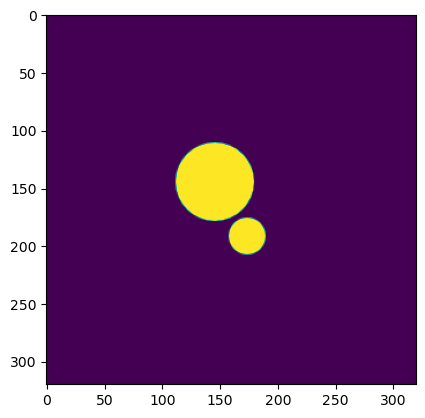
\includegraphics[width=0.35\linewidth]{papers/ct/images/img_recon.png}}
	\subfigure[Beispielbild Radon-transformiert.]{\label{ct:fig:radon}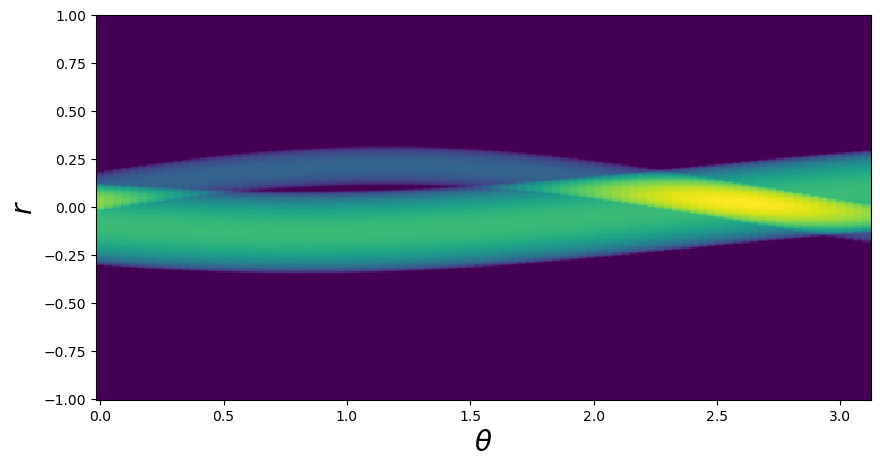
\includegraphics[width=0.55\linewidth]{papers/ct/images/radon.png}}
	\caption{Das Beispielbild und deren Radon-Transformation.}
\end{figure}


Die Rückprojektion in der Praxis verwendet nur eine endliche Anzahl von Werten. Dies führt dazu, dass die Rückprojektion nicht mit einem Integral berechnet werden kann, sondern mit einer Summe approximiert werden muss. 
Die kontinuierliche Variable $\theta$ wird in der diskreten Umgebung der Rückprojektion mit der diskreten Variable $\theta_i$, die sich auf die Winkel ${k\pi/N: 0\le k \le N-1}$ beschränkt, ersetzt. Diese Diskretisierung wird mit 
\begin{equation}\label{ct:discreteBP}
		\mathscr{B}_Dh(x, y) = \biggl(\dfrac{1}{N}\biggr)\sum_{k=0}^{N-1} h(x\cos(k\pi/N)+y\sin(k\pi/N), k\pi/N)
\end{equation}
beschrieben, wobei $k\pi/N$ mit $\theta_i$ zur Übersichtlichkeit ersetzt werden kann und somit resultiert
\begin{equation}\label{ct:discreteBP_w_theta}
	\mathscr{B}_Dh(x, y) = \biggl(\dfrac{1}{N}\biggr)\sum_{k=0}^{N-1} h(x\cos(\theta_i)+y\sin(\theta_i), \theta_i).
\end{equation}
Das Bild, welches durch den Scanner erhalten wird, wird in Abbildung \ref{ct:fig:radon} rechts gezeigt.
Auf das Bild des Scanners wird zunächst die Rückprojektion angewendet. Dies führt dazu, dass das Bild eine \glqq verschmierte\grqq{} Version des Beispielbildes wird, was in der Abbildung \ref{ct:fig:bp} gezeigt wird.

\begin{figure}
	\centering
	\subfigure[Die Rückprojektion.]{\label{ct:fig:bp}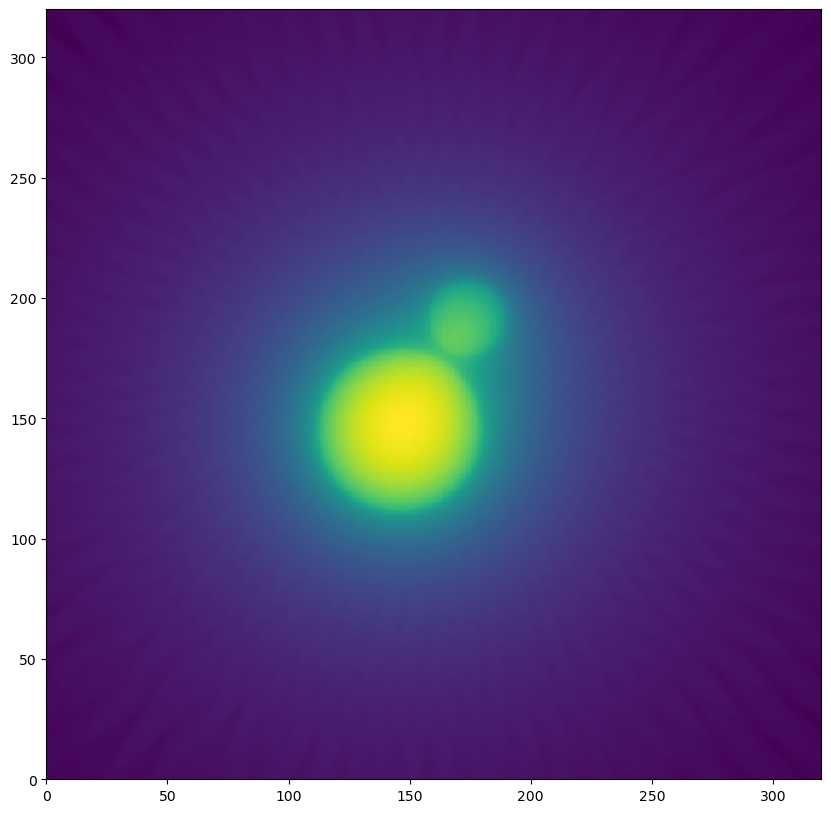
\includegraphics[width=0.45\linewidth]{papers/ct/images/bp.png}}
	\subfigure[Die gefilterte Rückprojektion.]{\label{ct:fig:fbp}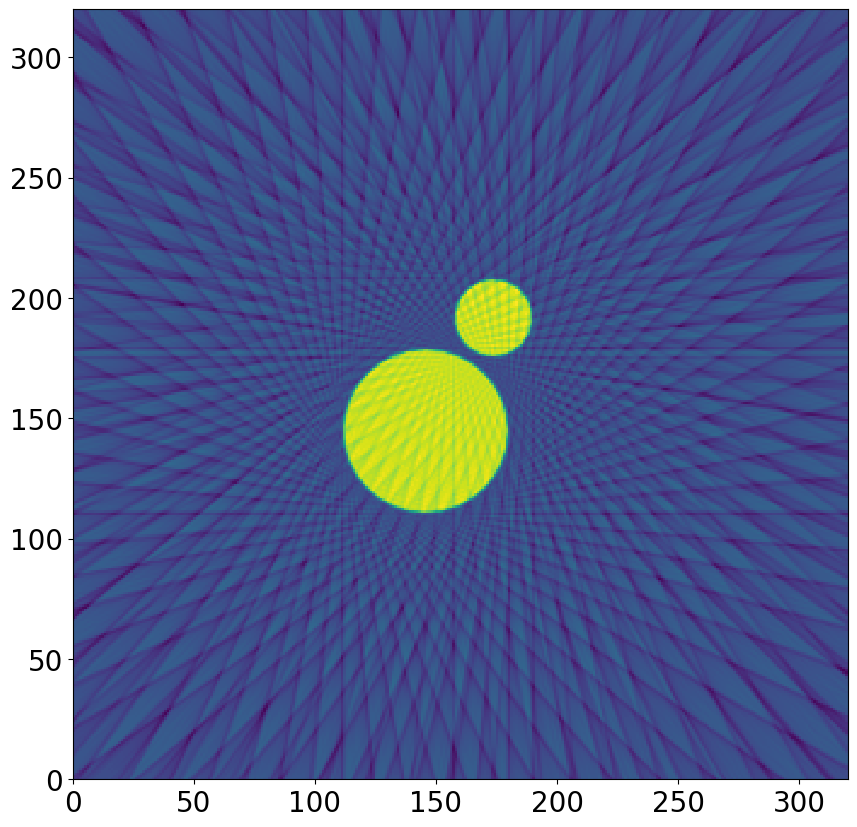
\includegraphics[width=0.45\linewidth]{papers/ct/images/fbp.png}}
	\caption{Die Rückprojektion und die gefilterte Rückprojektion des Beispielbildes.}
\end{figure}

Damit ein ungeglättetes Bild resultiert, wird die gefilterte Rückprojektion angewendet. Dabei wird als erstes das Bild des Scanners, ersichtlich in Abbildung \ref{ct:fig:radon}, Fourier-transformiert. Danach wird die Filterung mit $|S|$ durchgeführt und die inverse Fourier-Transformation davon gebildet. Schliesslich wird noch die Rückprojektion durchgeführt, was zur gefilterten Rückprojektion führt. 

Im Bild sind noch gewisse Artefakte ersichtlich, die sich durch Geraden im Bild zeigen. Diese Artefakte kommen daher, dass die Winkelauflösung begrenzt ist. In der Abbildung \ref{ct:fig:res} werden noch zwei Rekonstruktionen gezeigt, die einerseits eine tiefere Winkelauflösung und andererseits eine noch höhere Auflösung darstellen.

\begin{figure}
	\centering
	\subfigure[10° Auflösung.]{\label{ct:fig:lowRes}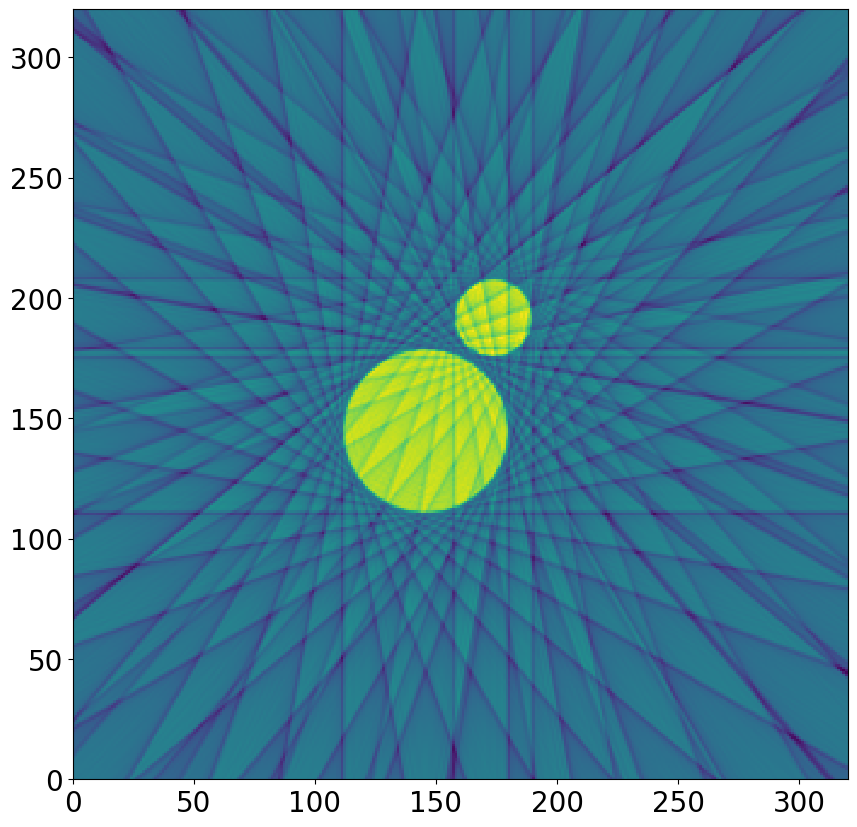
\includegraphics[width=0.45\linewidth]{papers/ct/images/fbp_low.png}}
	\subfigure[1° Auflösung.]{\label{ct:fig:highRes}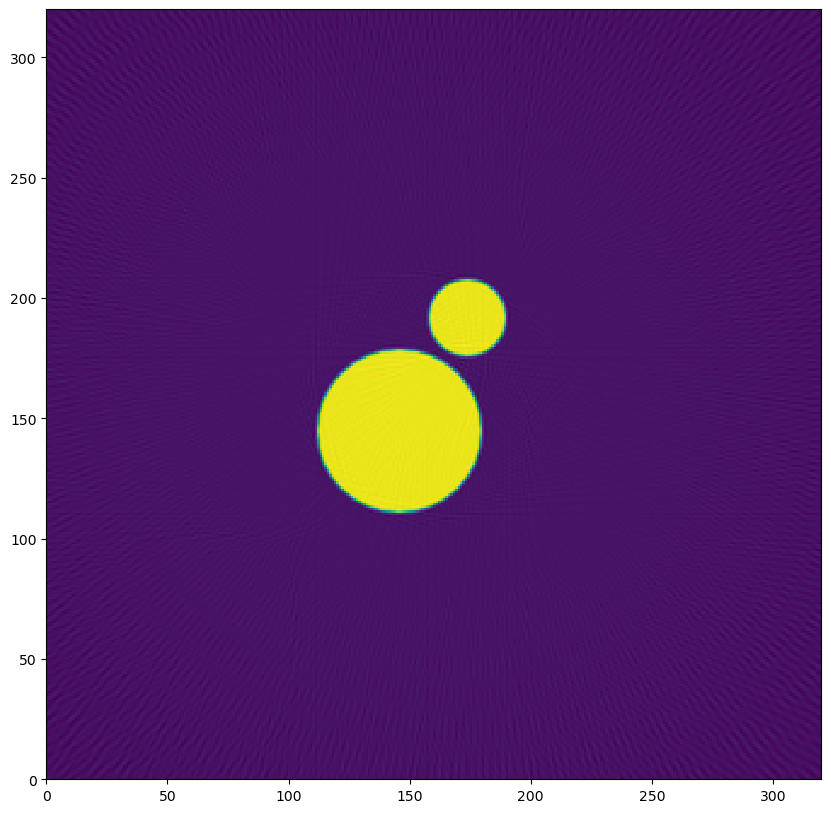
\includegraphics[width=0.45\linewidth]{papers/ct/images/fbp_high.png}}
	\caption{Die gefilterte Rückprojektion mit verschiedenen Auflösungen.}
	\label{ct:fig:res}
\end{figure}










